\chapter{Opdracht}

\section{Introductie}

Het bedrijf Shop2market is een software development bedrijf in de business-to-business sector. De organisatie helpt webwinkels online adverteren met als doelstelling de winstgevendheid van online advertenties te maximaliseren. Shop2market is ontstaan nadat duidelijk werd dat veel bedrijven niet de technologische middelen of kennis in huis hebben om zelfstandig te kunnen starten met adverteren. Zo blijkt uit interactie met klanten dat velen vrezen voor hoge kosten. Volgens mede opdrichter van Shop2market Matthijs Jorissen, komt dit door het gebrek aan transparantie en het complexe landschap dat is gecreeërd door de grootte hoeveelheid bedrijven.

Voor alsnog diende shop2market als een IT oplossing ondersteunend aan het adviesbedrijf. Het merendeel van deze klanten zijn webwinkels in het A segment. Maar omdat de integratie met een webwinkel vaak maatwerk opleverde duurde een integratie gemiddeld zes tot acht maanden. Dit heeft een hoop klanten opgeleverd maar bleef erg onderhoudsintensief en hinderde de groei van Shop2market.

Hierdoor heeft het bedrijf zijn strategie opnieuw gedefinieerd. Hieruit kwam dat het webwinkels in het midden en klein bedrijf op internationaal niveau wil kunnen bedienen. De gewenste groei moet mogelijk worden gemaakt doordat webwinkel platformen zoals SEOShop, Shopify en Magento een gestandaardiseerde integratie mogelijk maken. Hierdoor wordt een webwinkel geïntegreerd in slechts enkele minuten.

Adcurve is een online dienst die is ontwikkeld in 2015 door Shop2market. Met de ervaring vanuit de adviesorganisatie zijn veel processen vertaald naar functionaliteiten om een self-service applicatie mogelijk te maken. De eerste beta versie van Adcurve is in de zomer van 2015 gelanceerd voor webwinkels die gebruik maken webwinkelplatformen als SEOshop of Magento. Hiermee kunnen webwinkels volledig zelfstandig aan de slag.

Webwinkel eigenaren kunnen nu hun producten gemakkelijk adverteren via zogeheten publishers. Dit zijn bedrijven die de advertenties publiseren. Bijvoorbeeld ingekochte zoekresultaten op Google via Google Adwords, op prijsvergelijkers en affiliate via Beslist.nl of Zanox. Maar ook Marktplaatsen zoals Amazon.com en Google Shopping maken hier onderdeel van uit.

Vervolgens biedt Adcurve de mogelijkheid om de winstgevendheid van de advertenties in te zien en hierop te handelen\footnote{Dit word ook wel "Actionable insights" genoemd in tegenstelling tot enkel het bieden van inzicht zoals Analytics tools}. Dit is mogelijk doordat Adcurve een partij is tussen de webwinkel en publishers.

\section{Aanleiding} % de aanleiding tot de opdracht

Het afgelopen jaar zijn de meeste basis functionaliteiten ontwikkeld zoals registratie, een App Store voor publishers, datavisualisaties en advertentie beheer. Momenteel is het ontwikkelteam gefocused om meer publishers te integereren. Dit is strategisch om meer landen en industriën te kunnen ondersteunen en zo meer klanten te krijgen. Zodra een gebruiker een publisher installeerd vindt er een volledige integratie plaats. Voor de webwinkel word de afkomstigheid van bezoekers en bestellingen gemeten. In combinatie met de advertentiekosten van publishers worden de nodige statistieken berekend.

% FIXME: Omdat de belangrijkste functionaliteiten zijn gebaseerd op statistieken is het belangrijk dat berekeningen op tijd klaar zijn.
Sinds het aantal data integraties met publishers is gegroeid, ervaart het team problemen met het databeheer hiervan. Er is hierdoor een een toenemende wens ontstaan om de huidige oplossing te herzien. Dit moet de gewenste groei van Adcurve onderstuenen en ruimte bieden om functionaliteiten betrouwbaarder en te maken.

\section{Context van het bedrijf} % beschrijving van de organisatie van de opdrachtgever en de plaats van de student daarin

Shop2market is gevestigd in Hilversum en heeft tussen de 15 en 20 werknemers. De organisatie structuur kan naar de theorie van \autocite{mintzberg} worden omschreven als een Adhocracy: “Door de innovatieve aard van projecten is een organisatie gebaat bij flexibiliteit. Een formele hiërarchische structuur werkt daardoor minder goed.” Dit is herkenbaar en valt terug te leiden naar de professionele houding die van werknemers word verwacht. Er word autonomie gegeven om zelf structuur aan te brengen wanneer dit nodig is.

De software ontwikkeling valt onder leiding van M. Jorissen. In nauwe samenwerking met M. Gill zijn zij verantwoordelijk voor de project analyse en planning. Het development team bestaat uit zes ontwikkelaars waaronder één ontwerper D.  De architectuur wordt geleid door S. Pogrebnyak. Dit team is verantwoordelijk voor het uitwerken en oplossen van projecten. Hierbij word gebruik gemaakt van een aantal methodieken en gewoontes vanuit Agile-softwareontwikkeling, waaronder: Kanban, Daily standup, Retrospectives, Extreme Programming (XP), Test Driven Development (TDD) en Continuous integration (CI).

Ondanks dat er in de werkwijze vaak een uitgebreide planning of requirements analyse ontbreekt, word de productiviteit en software kwaliteit toch bewaakt door de principes uit XP zoals TDD en refactoring \footnote{“Code refactoring is het proces waarbij de structuur van bestaande code word gewijzigd zonder de functionaliteit te wijzigen”…“dit komt ten goede aan de onderhoudbaarheid van code, en creëert nieuwe architectuur of object modellen om code makkelijker te kunnen uitbreiden met nieuwe functionaliteiten“ \parencite{refactoring}}. Hierdoor kan het team zich veroorloven om alleen voor de huidige situatie en problemen te ontwerpen. Veel planning is hierdoor niet aanwezig en technische implementatie komt vooral tot stand door TDD, brainstorm sessies, en de vrijheid om te proberen en fouten te maken.

\begin{figure}[h]
    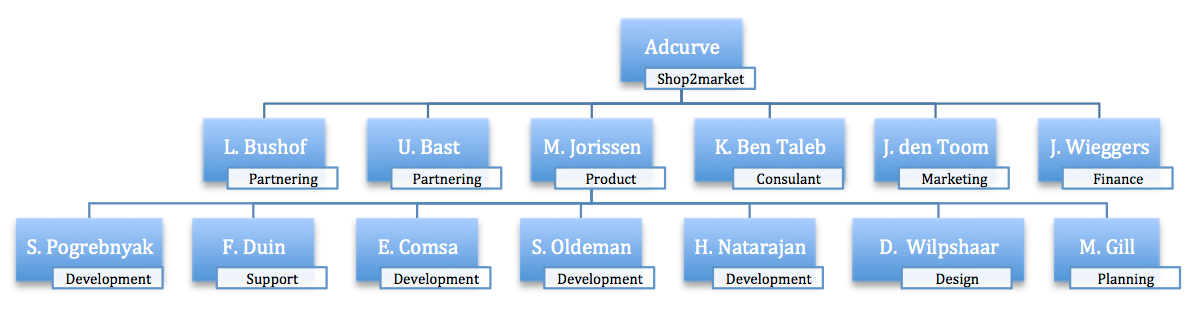
\includegraphics[width=1\textwidth]{organisation_structure.png}
    \caption{Organogram waarin de relatie tussen Shop2market en Adcurve zichtbaar is.}
    \label{fig:orgchart}
\end{figure}

\section{De kwestie} % een kwestie (aanleiding, het op te lossen probleem, de te vervullen behoefte of de te benutten kans);

Statistieken worden op dit moment dagelijks berekend voor de afgelopen dag. Dit wordt gestart wanneer alle databronnen aanwezig zijn, rond 10:00 CET en duurt tot ongeveer 16:00 CET. Met als resultaat dat niet alle functionaliteiten actueeel zijn tijdens kantooruren. Dit proces kan verder vertraagd raken wanneer berekeningen voor een eerdere dag opnieuw gestart zijn om een correctie uit te voeren.

% De tijd die het duurt om statistieken te berekenen is linear gestegen met de groei in webwinkels en de hoeveelheid geinstalleerde publishers. Het is daarom de wens om de oplossing te herzien.

\section{Doelstellingen} % de doelstellingen (wat moet na afloop van het afstudeerproject zijn bereikt);

Webwinkeleigenaren moeten kunnen handelen op actuele gegevens op basis van functionaliteiten in Adcurve die zijn gebaseerd op statestieken.

Webwinkeleigenaren maken beslissingen op actueele data uit statistieken doordat de functionaliteiten in Adcurve gebruik maken van statistieken die altijd up-to-date zijn.
Het herstel van fouten


Er moet een nieuwe oplossing worden ontwikkeld om statistieken te

Het nieuwe statistieken platform moet tijdig herstel mogelijk maken van onjuistheden. Ook moeten gebruikers functionaliteiten op basis van statistieken op tijd beschikbaar zijn voor de gebruikers. Dit moet mogelijk zijn door de snelheid waarmee berekeningen worden uitgevoerd.



\section{Deel producten}


% TODO: Het type opdracht kan worden omschreven als een product en ontwerp opdracht.


